\documentclass[dvipdfmx]{jsarticle}
\usepackage[dvipdfmx]{graphicx}
\usepackage{caption}
\usepackage{here}
\captionsetup[figure]{labelsep=period, labelfont=bf, justification=raggedright, singlelinecheck=off}

\begin{document}
    \begin{titlepage}
        \begin{center}
            \vspace*{180truept}
            {\Huge 技術書SNS 設計書}

            \vspace{160truept}
            {\Large グループメンバー}
            %なんか書かないといけないので適当に役割書いてます

            \vspace{20truept}
            {\Large バックエンド担当 \quad20-1-037-0112 穂積 優真}

            \vspace{10truept}
            {\Large フロントエンド担当 20-1-037-0027 實藤 敬太}
            {\Large }

            \vspace{160truept}
            \today
        \end{center}
    \end{titlepage}
    \newpage

    \section*{イントロダクション}
    \subsection*{\rm{作成者:穂積(バックエンド担当)}}
    \section{アプリケーションの目的}
    \newpage

    \section*{ユースケース図とユースケース記述}
    \subsection*{\rm{作成者:穂積(バックエンド担当)}}
        \begin{figure}[H]
            \begin{center}
                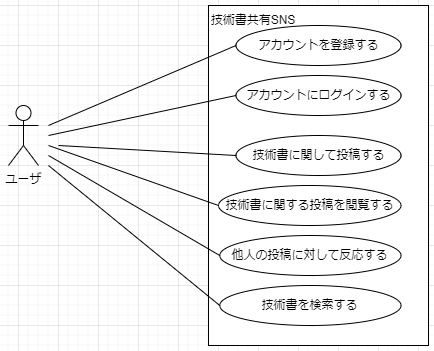
\includegraphics[scale=1.0,clip]{pictures/usecase.drawio_1.png}
            \end{center}
        \end{figure}

    \newpage
    
    \section*{ページ遷移図}
    \subsection*{\rm{作成者:ユースケース記述 穂積(バックエンド担当)}}
    \begin{figure}[H]
        \begin{center}
            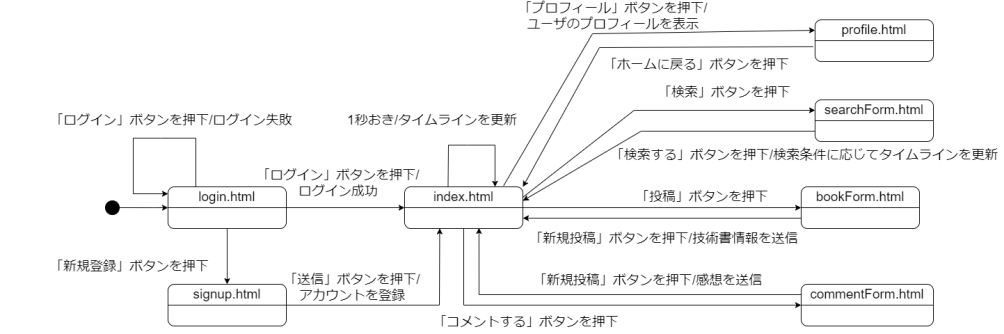
\includegraphics[scale=0.5,clip]{pictures/pageSenni_1.png}
        \end{center}
    \end{figure}

    \newpage

    \section*{試作ページ}
    \subsection*{\rm{作成者:穂積(バックエンド担当)\& 實藤(フロントエンド担当)}}
    \begin{figure}[H]
        \begin{center}
            \caption*{login.html}
            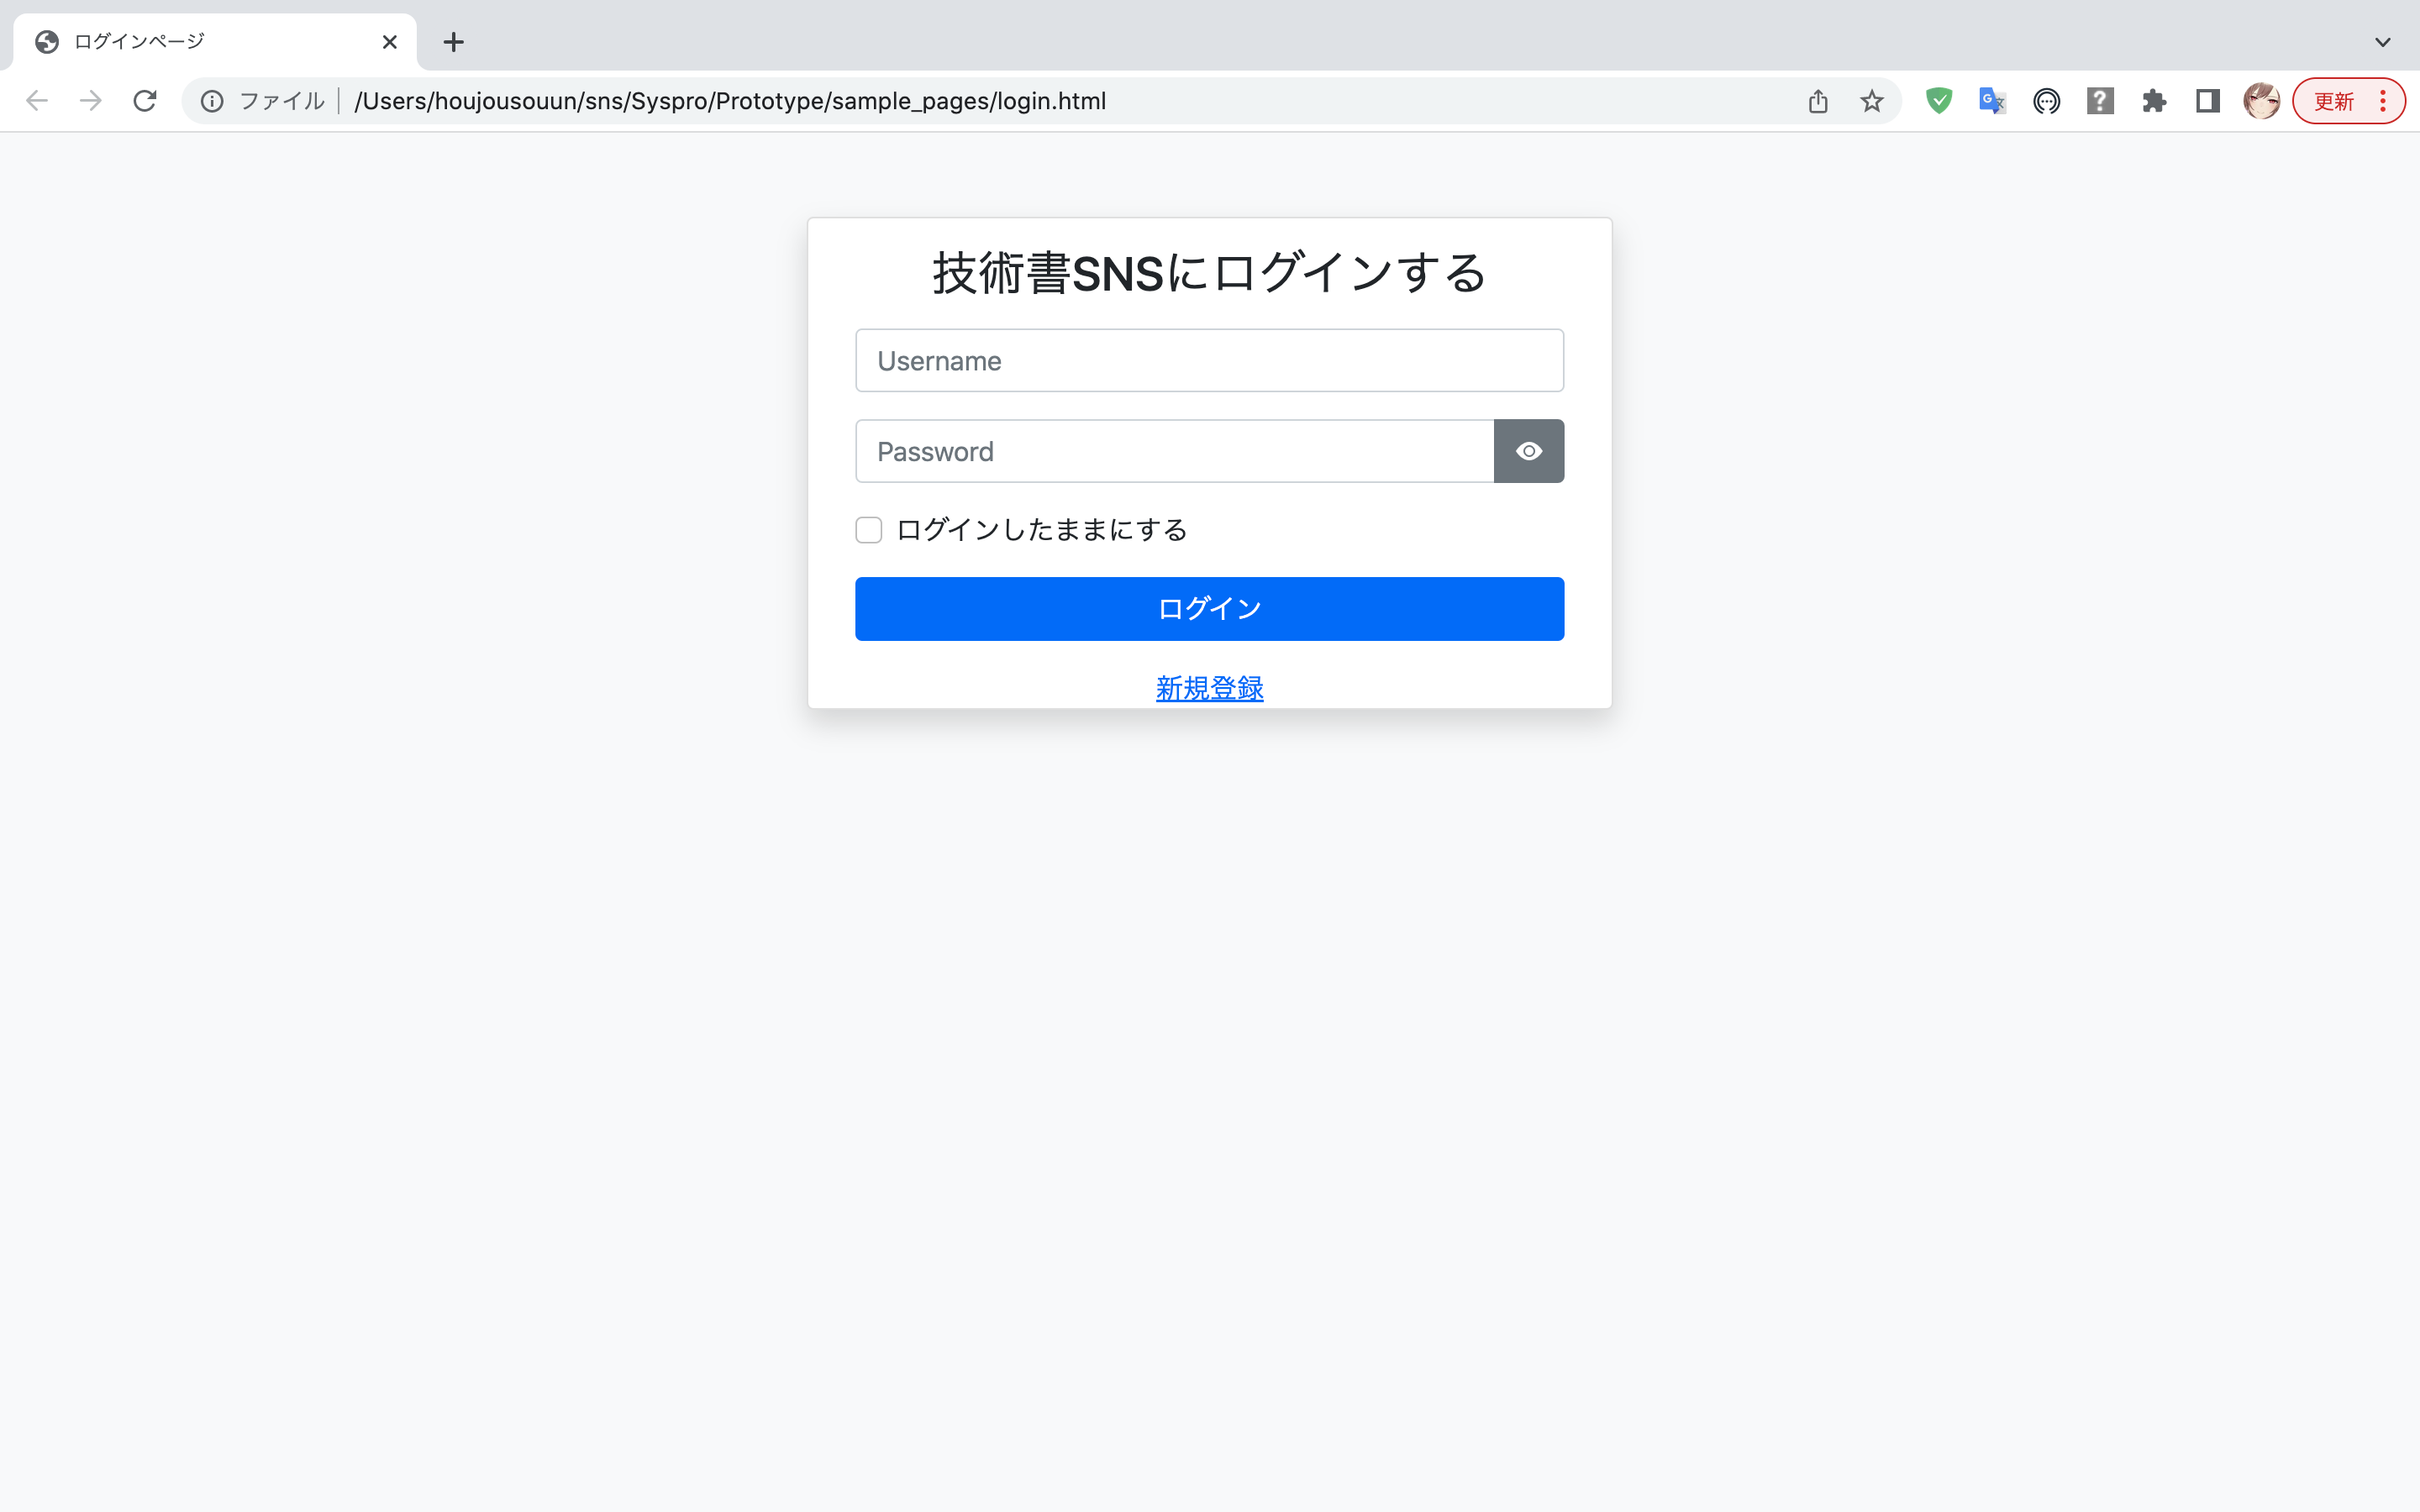
\includegraphics[scale=0.3,clip]{pictures/login.png}
        \end{center}
    \end{figure}

    \begin{figure}[H]
        \begin{center}
            \caption*{signup.html}
            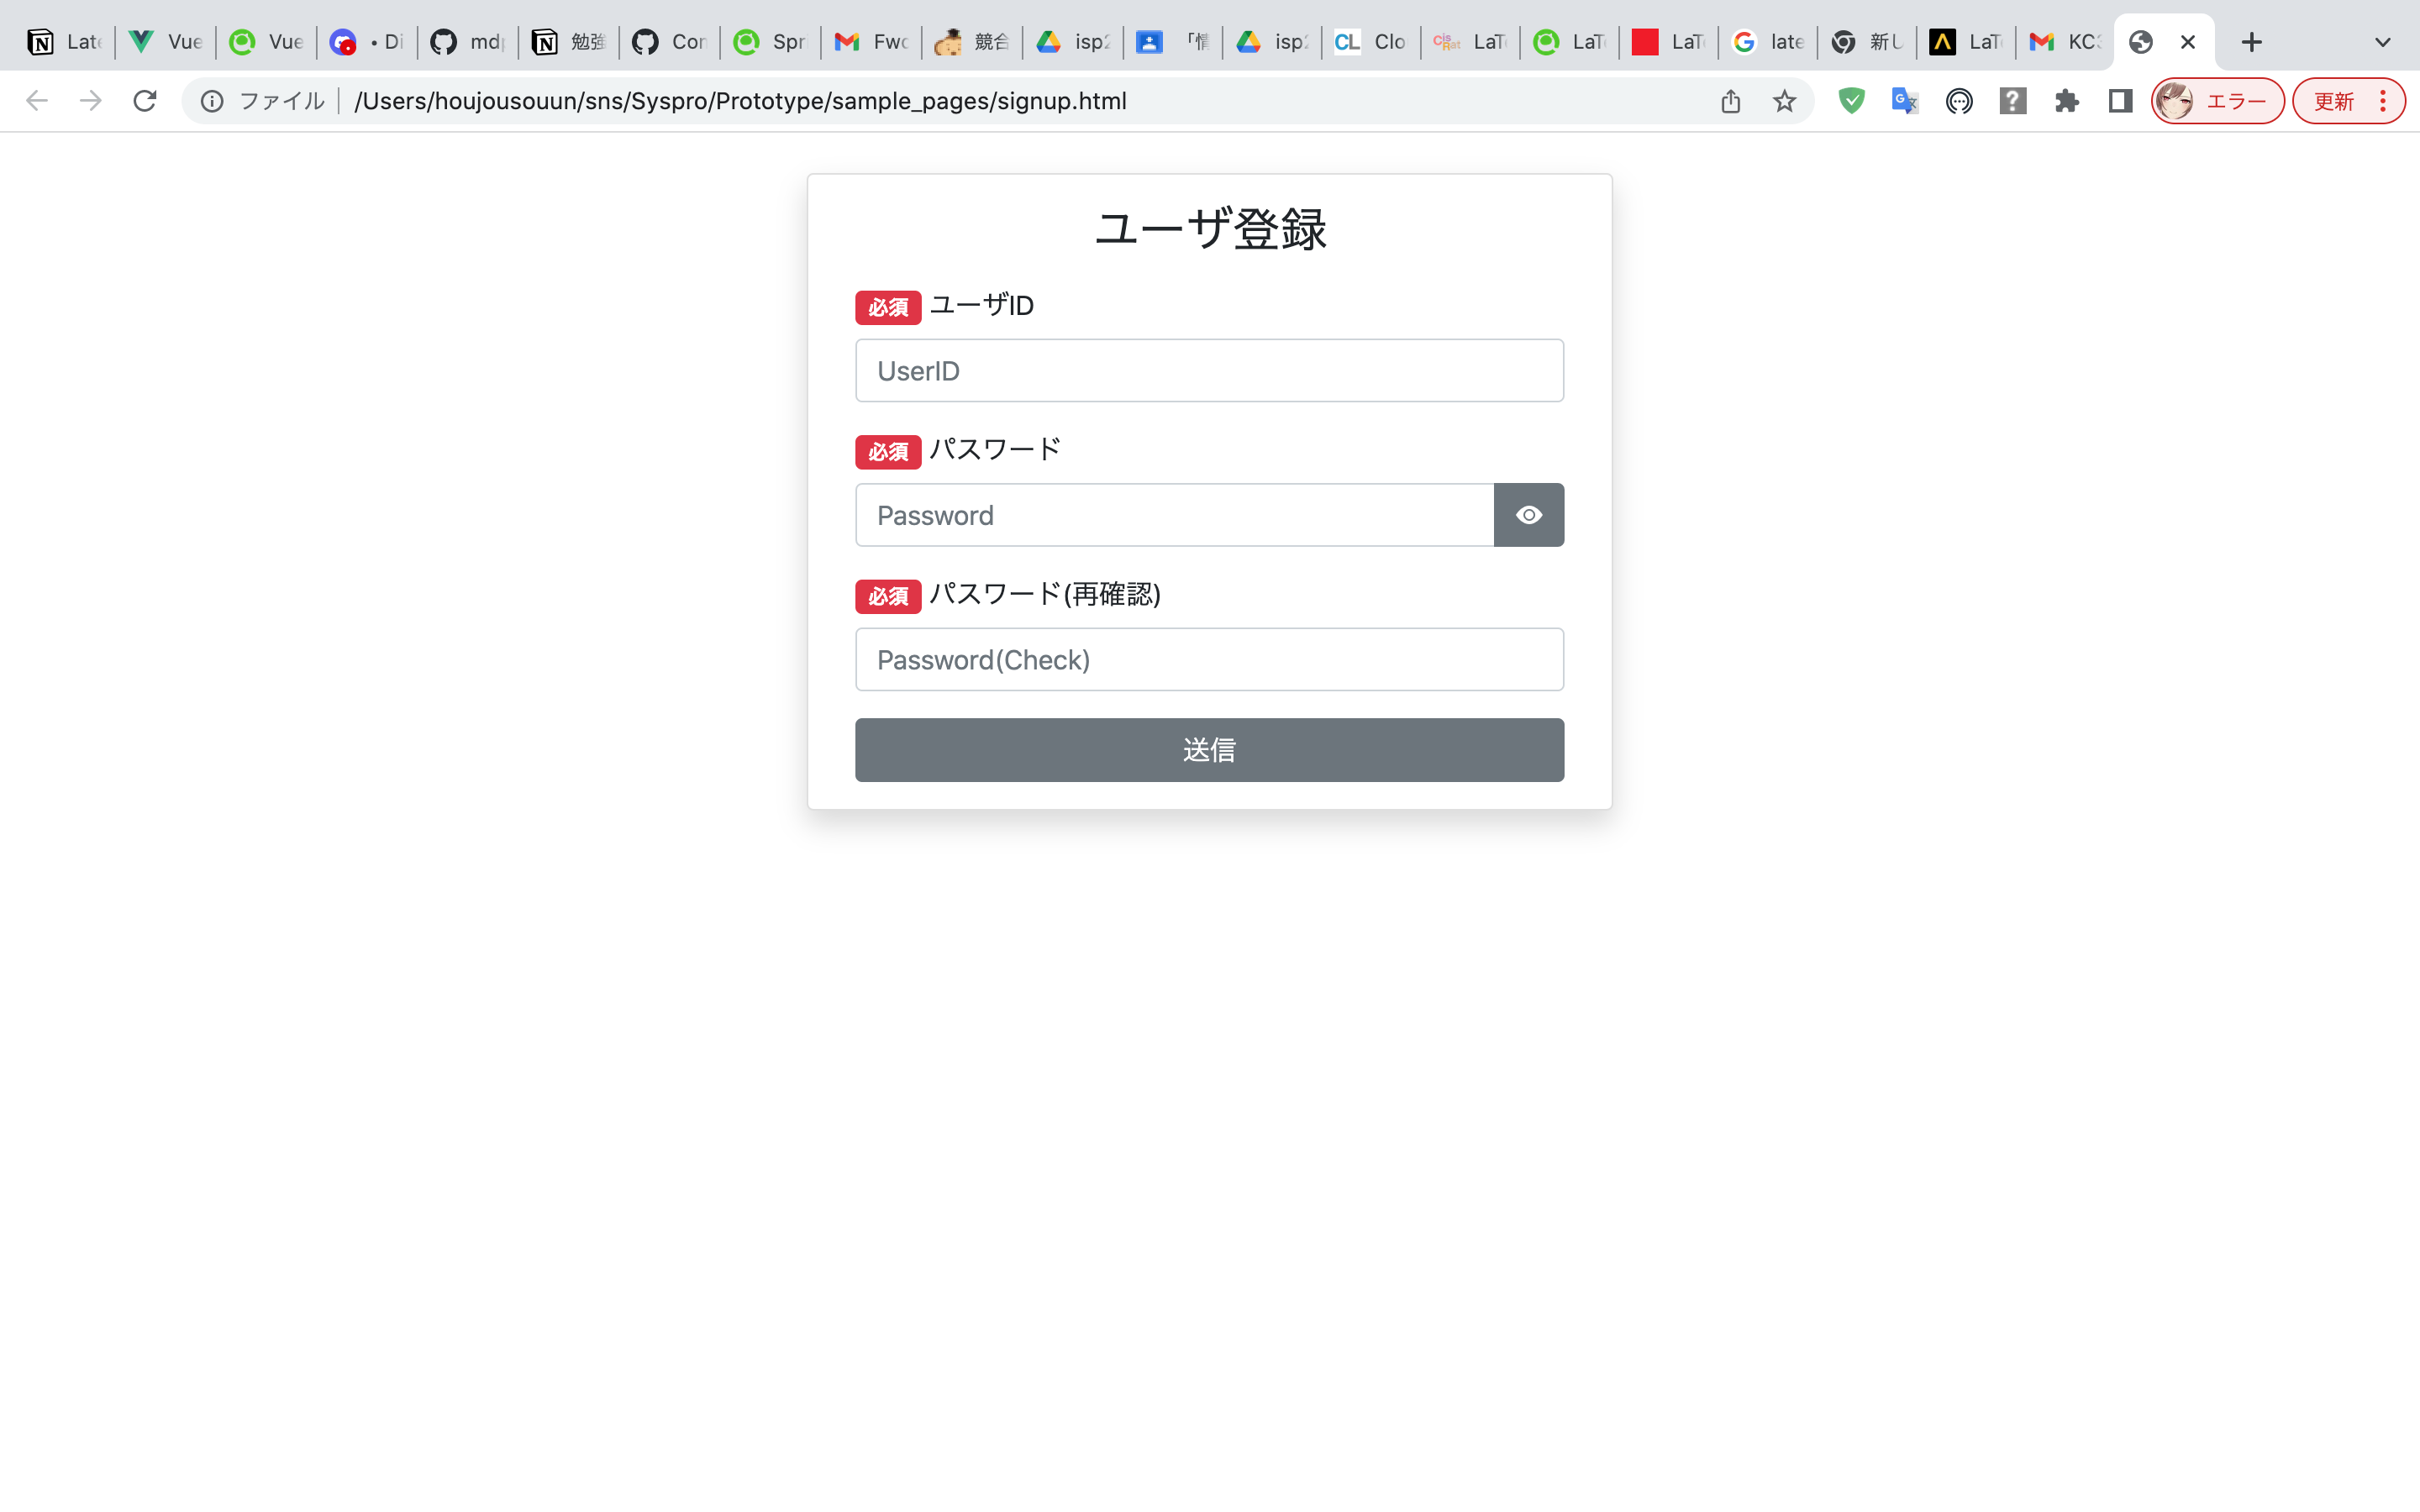
\includegraphics[scale=0.3,clip]{pictures/signup.png}
        \end{center}
    \end{figure}

    \begin{figure}[H]
        \begin{center}
            \caption*{index.html}
            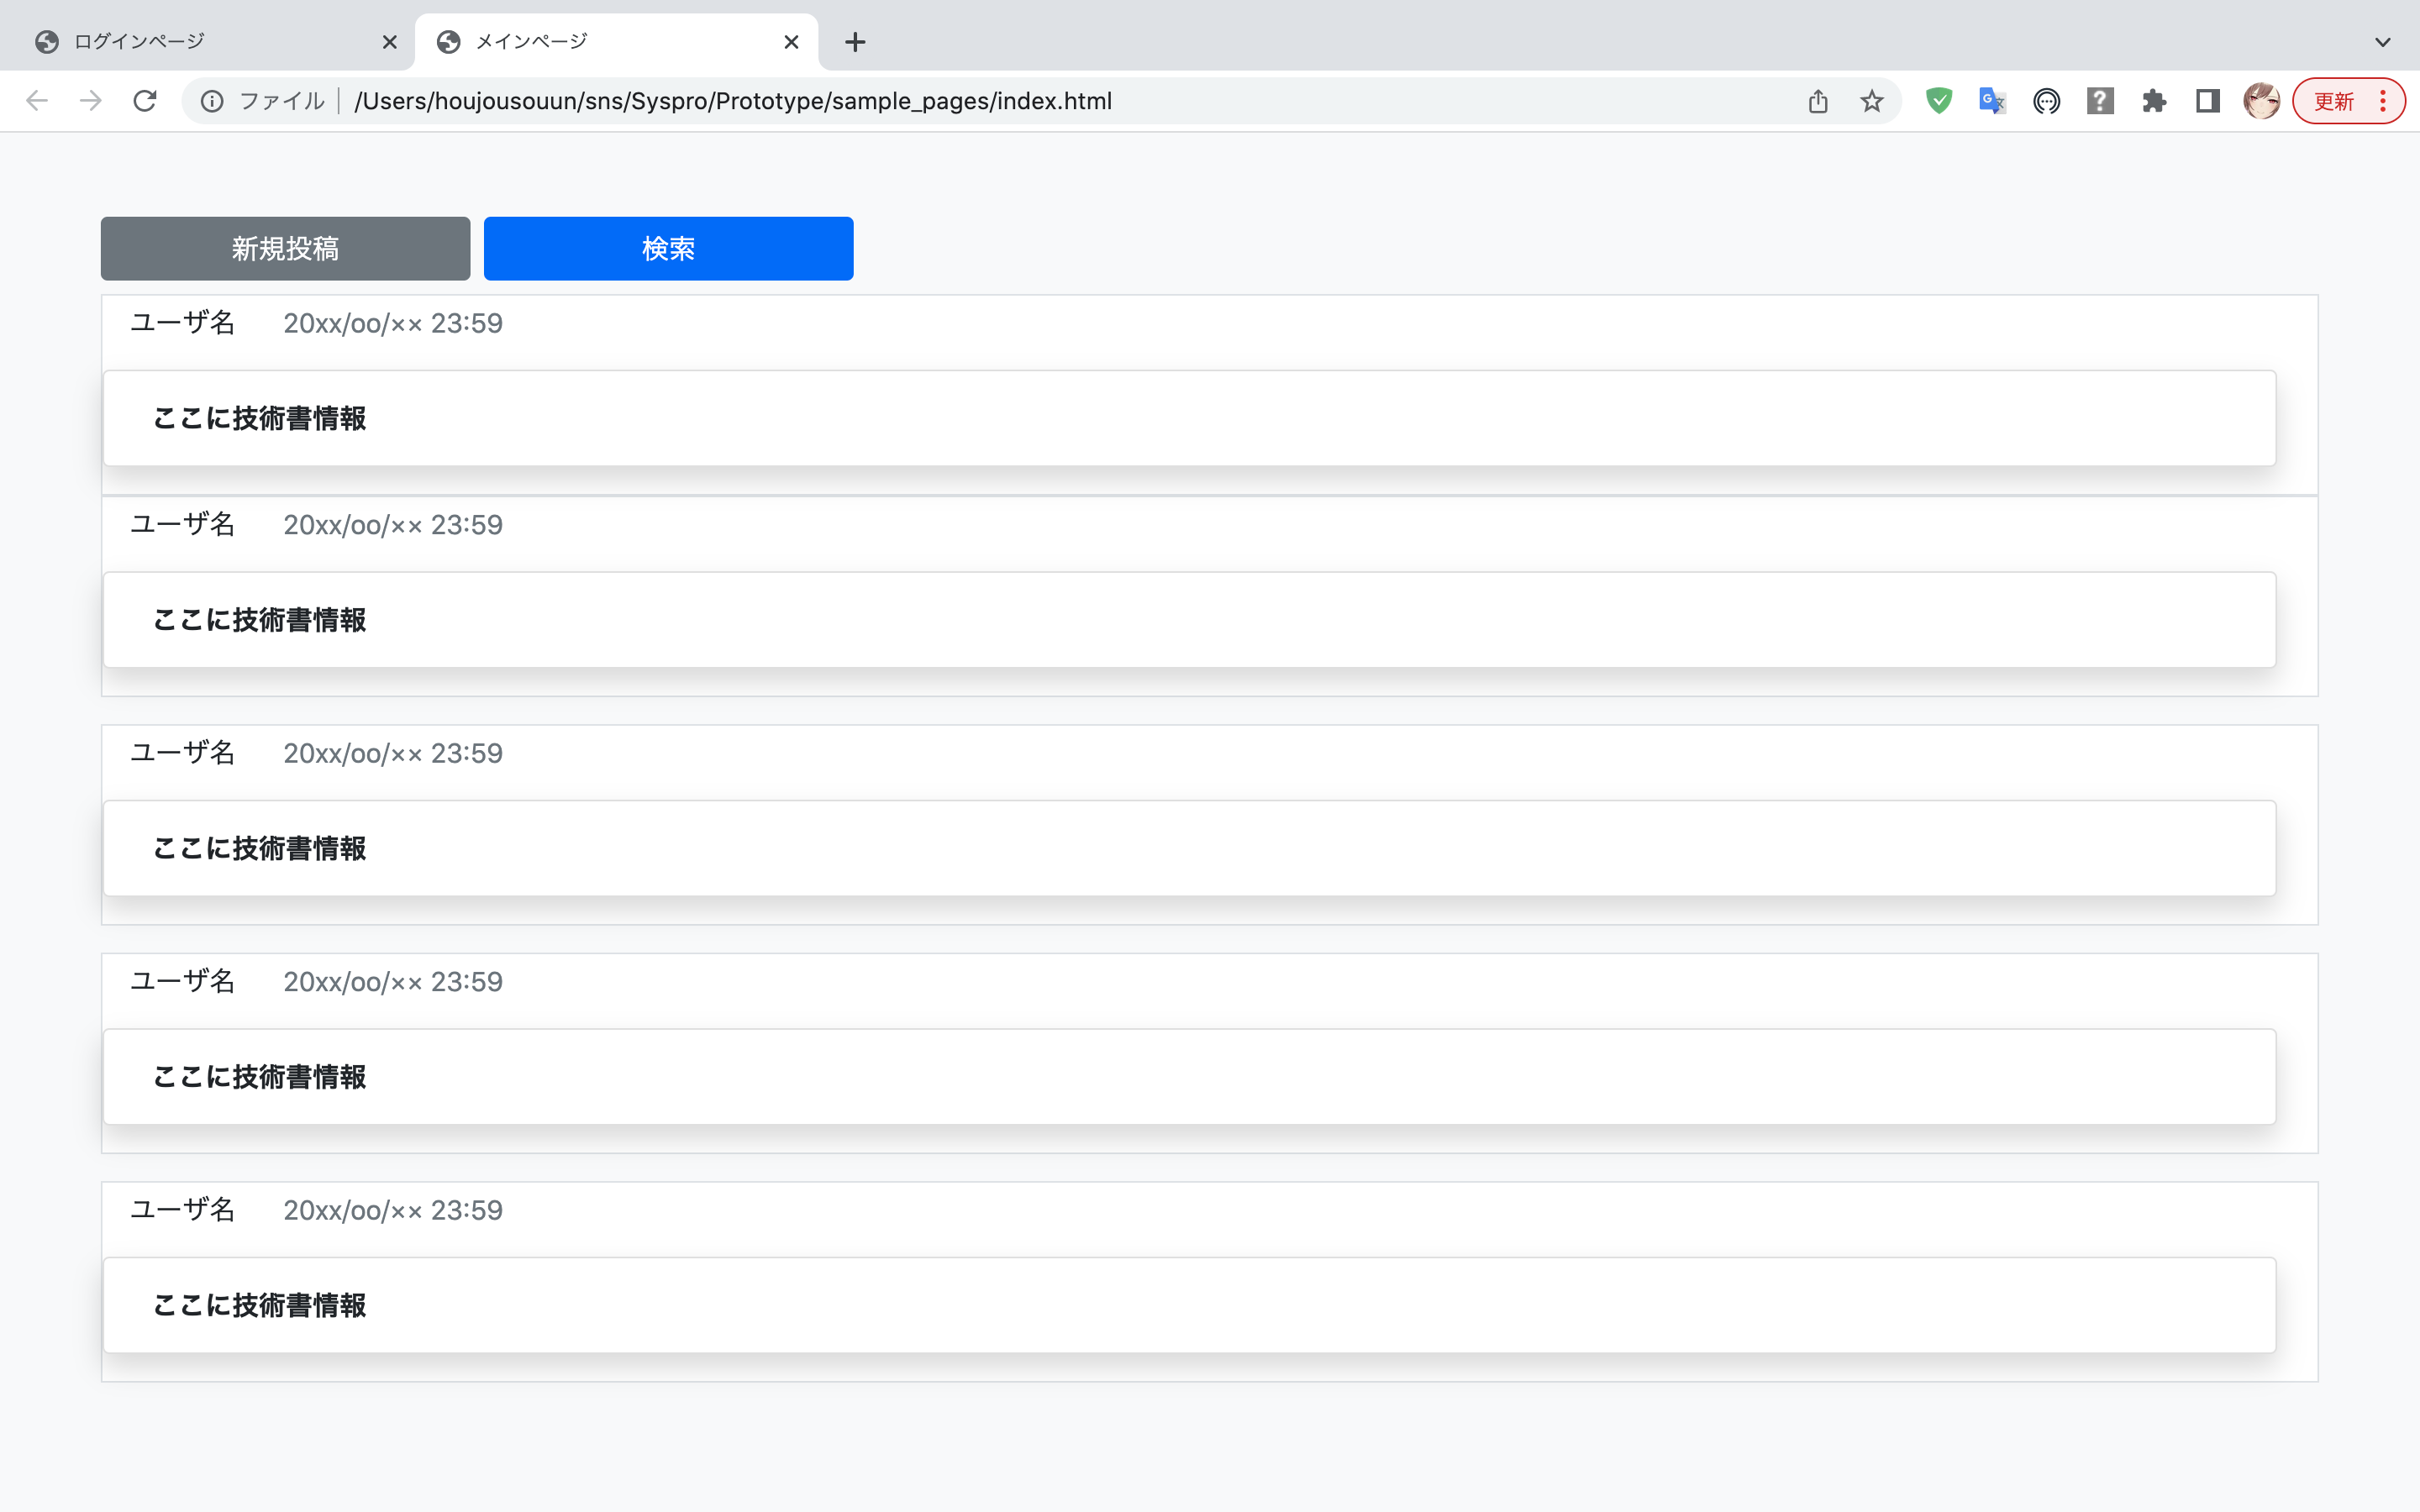
\includegraphics[scale=0.3,clip]{pictures/index.png}
        \end{center}
    \end{figure}

    \begin{figure}[H]
        \begin{center}
            \caption*{profile.html}
            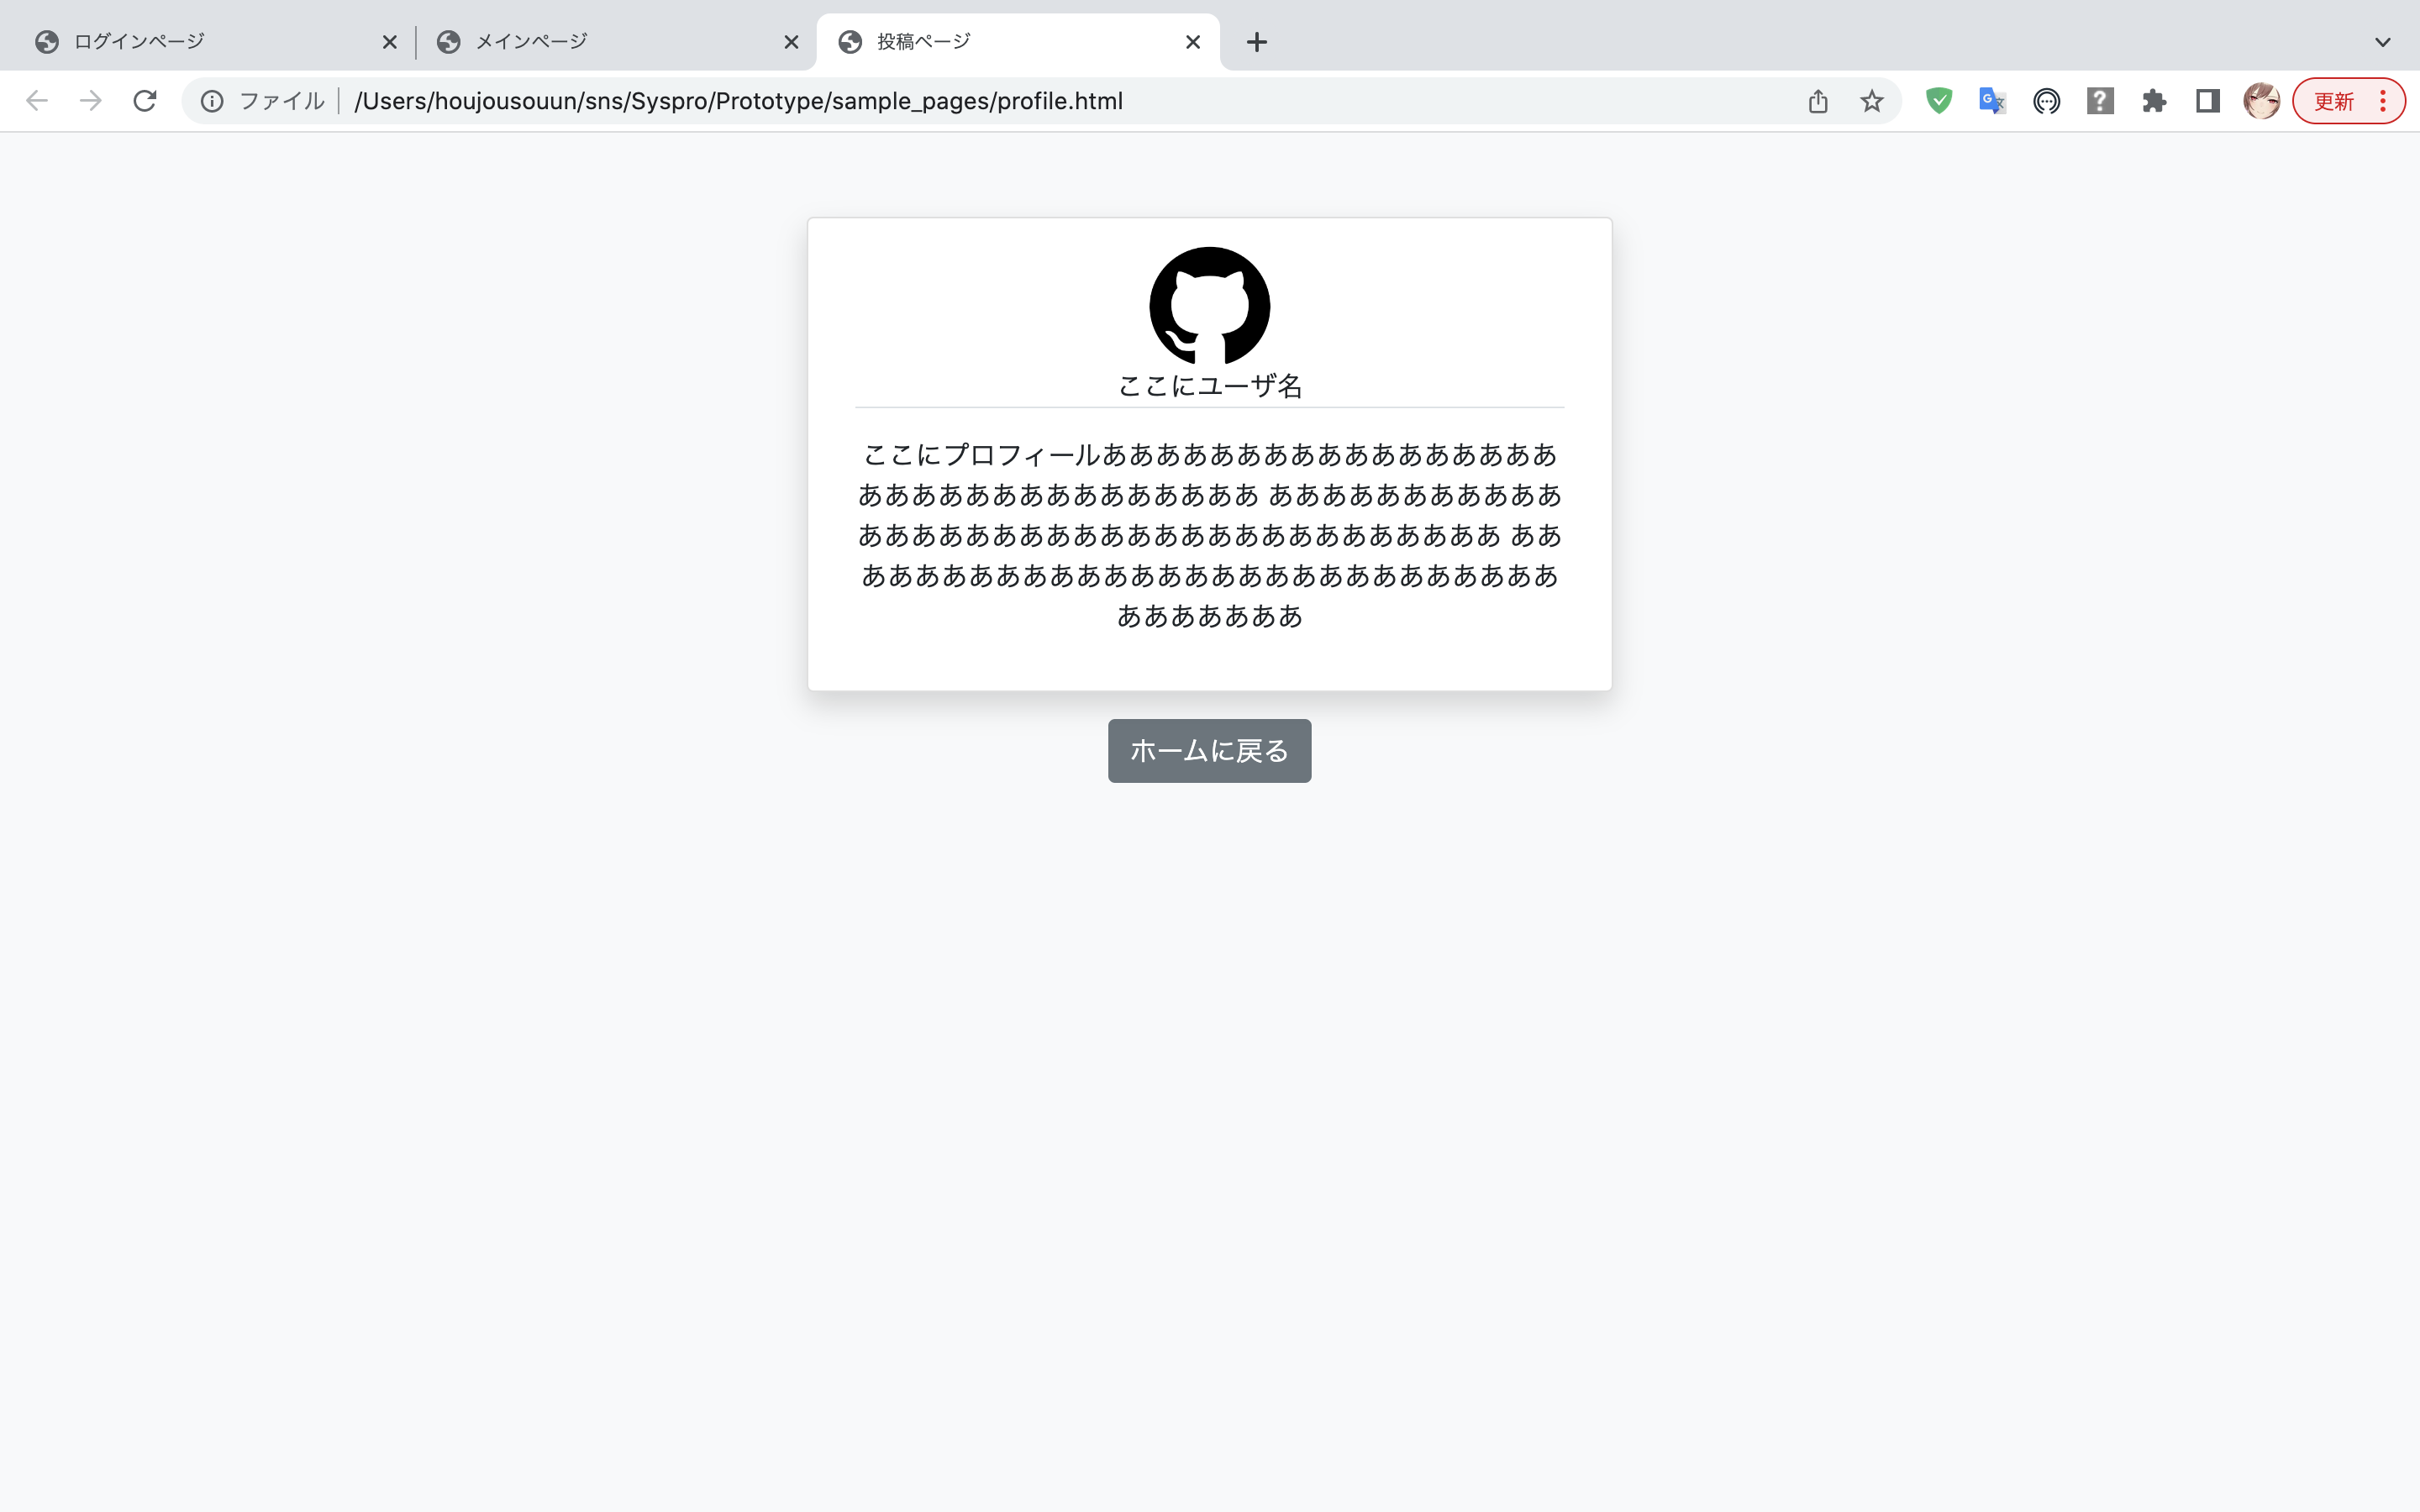
\includegraphics[scale=0.3,clip]{pictures/profile.png}
        \end{center}
    \end{figure}

    \begin{figure}[H]
        \begin{center}
            \caption*{searchForm.html}
            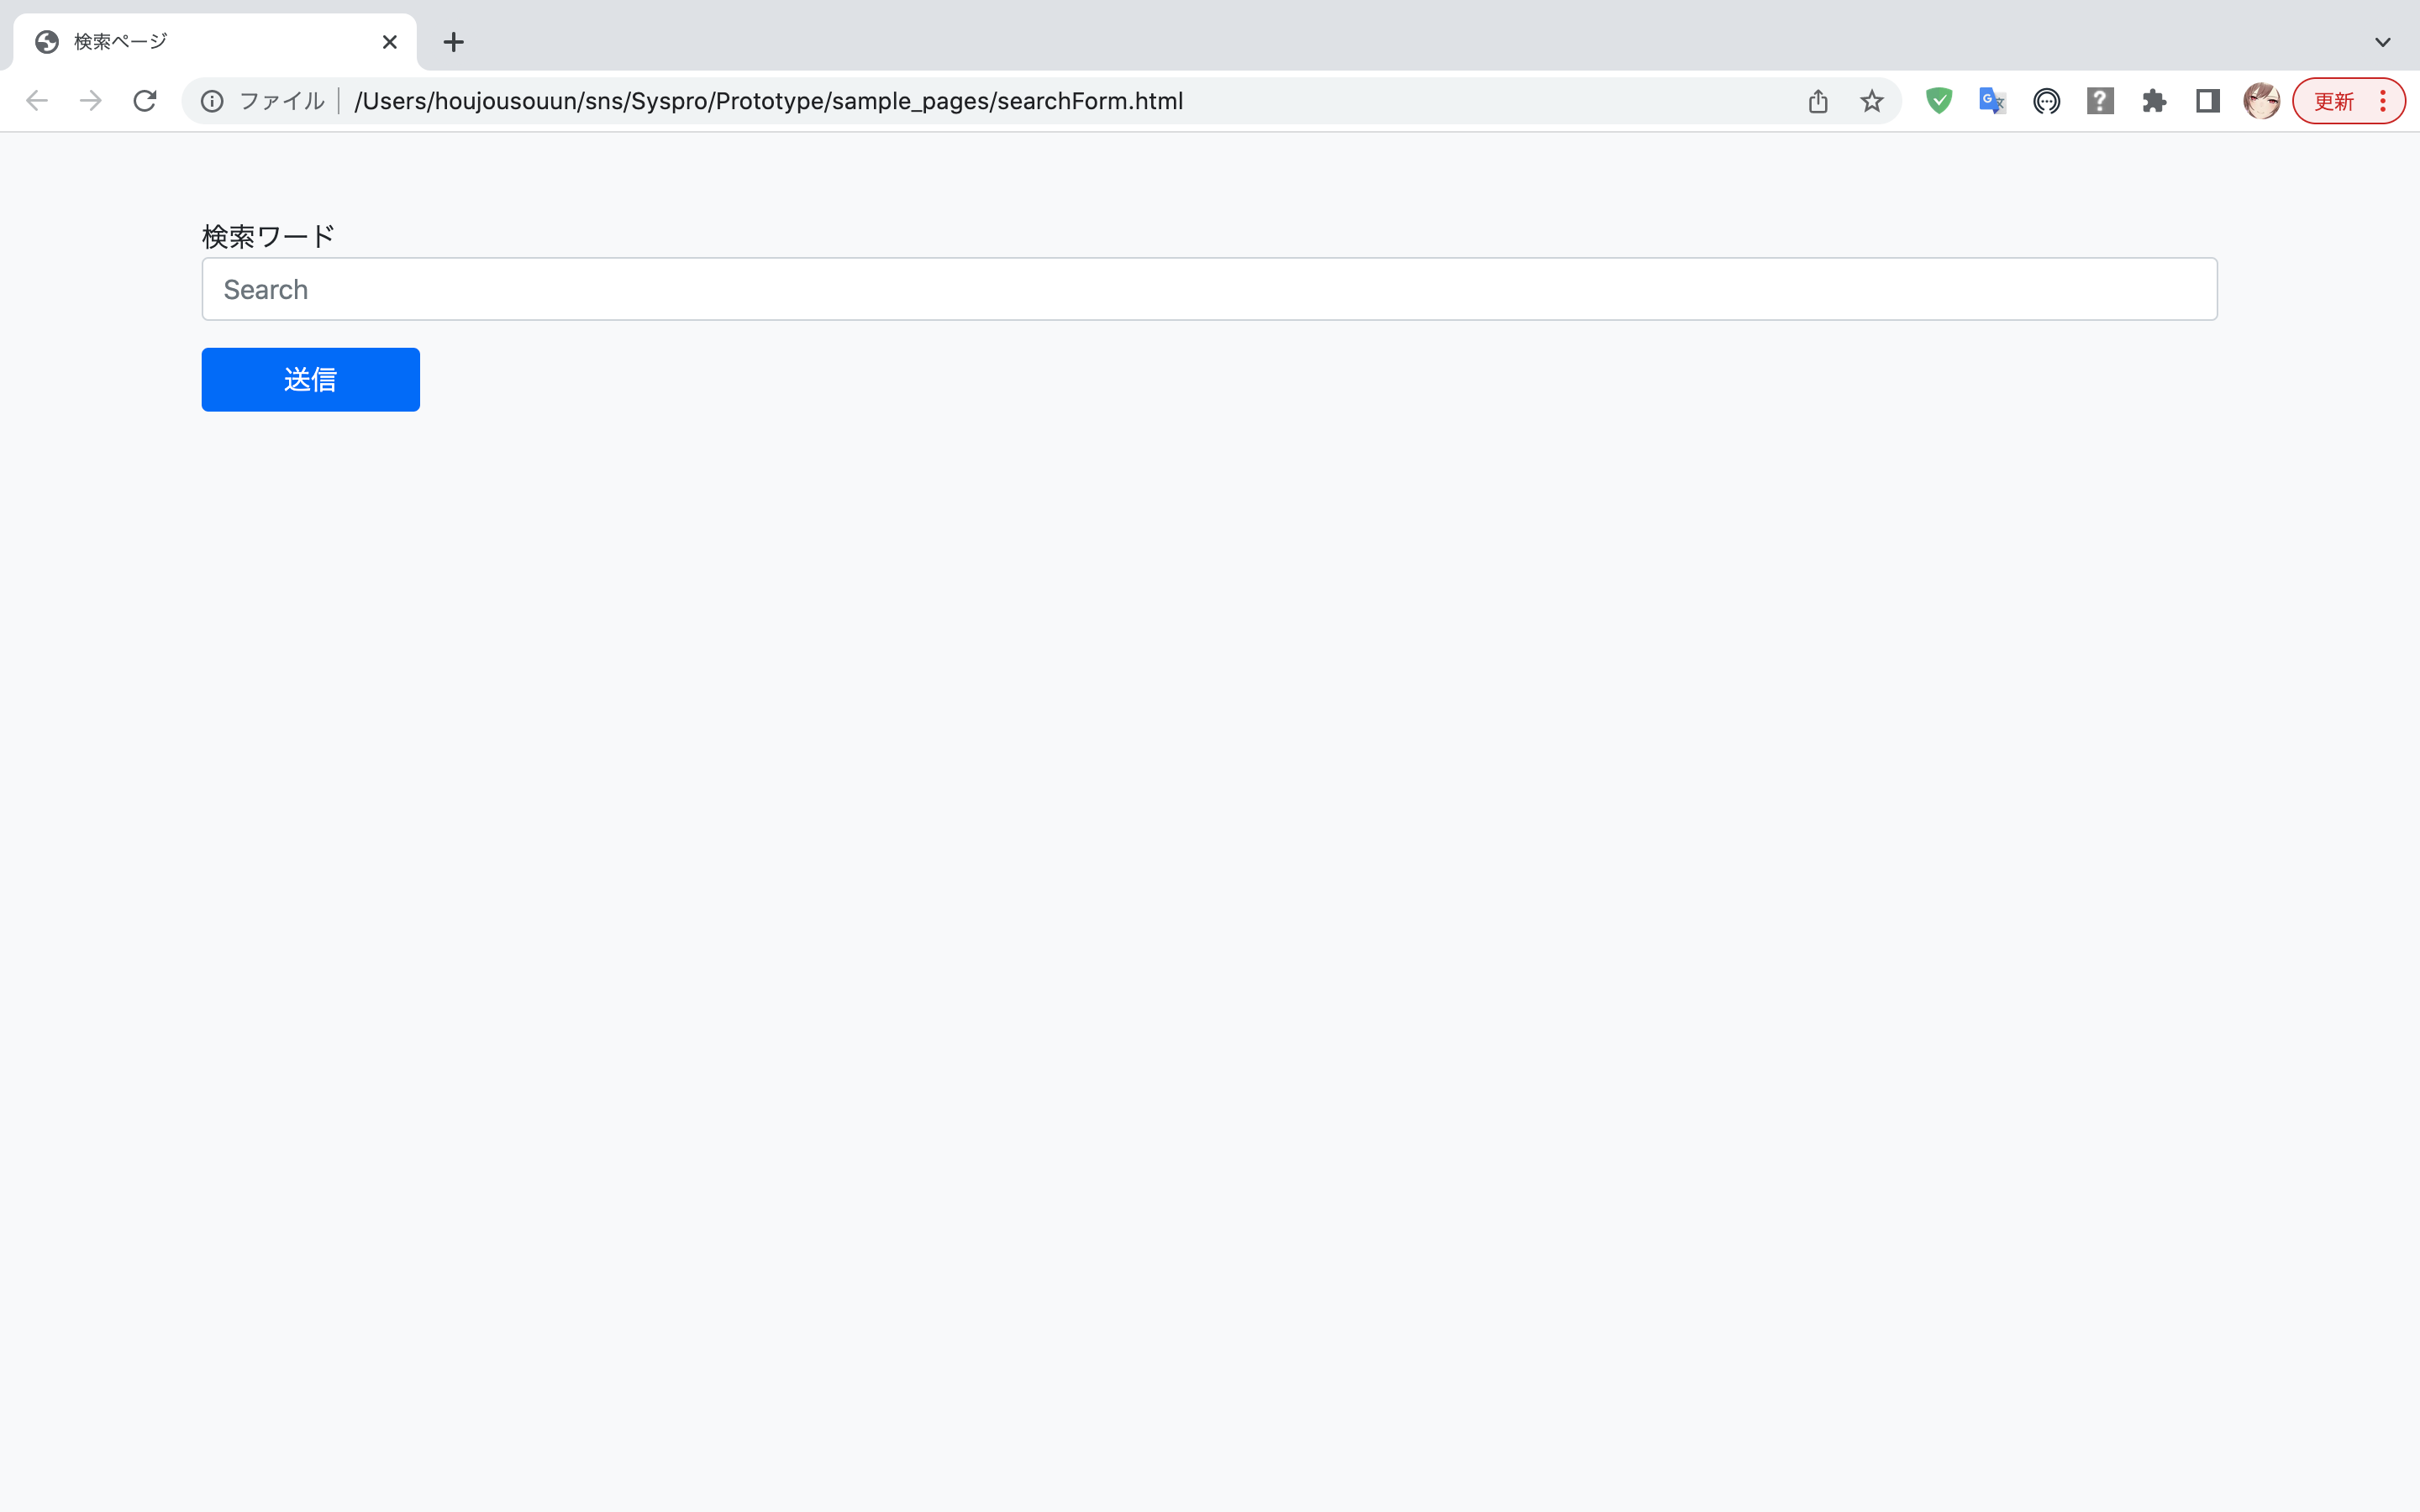
\includegraphics[scale=0.3,clip]{pictures/searchForm.png}
        \end{center}
    \end{figure}

    \begin{figure}[H]
        \begin{center}
            \caption*{bookForm.html}
            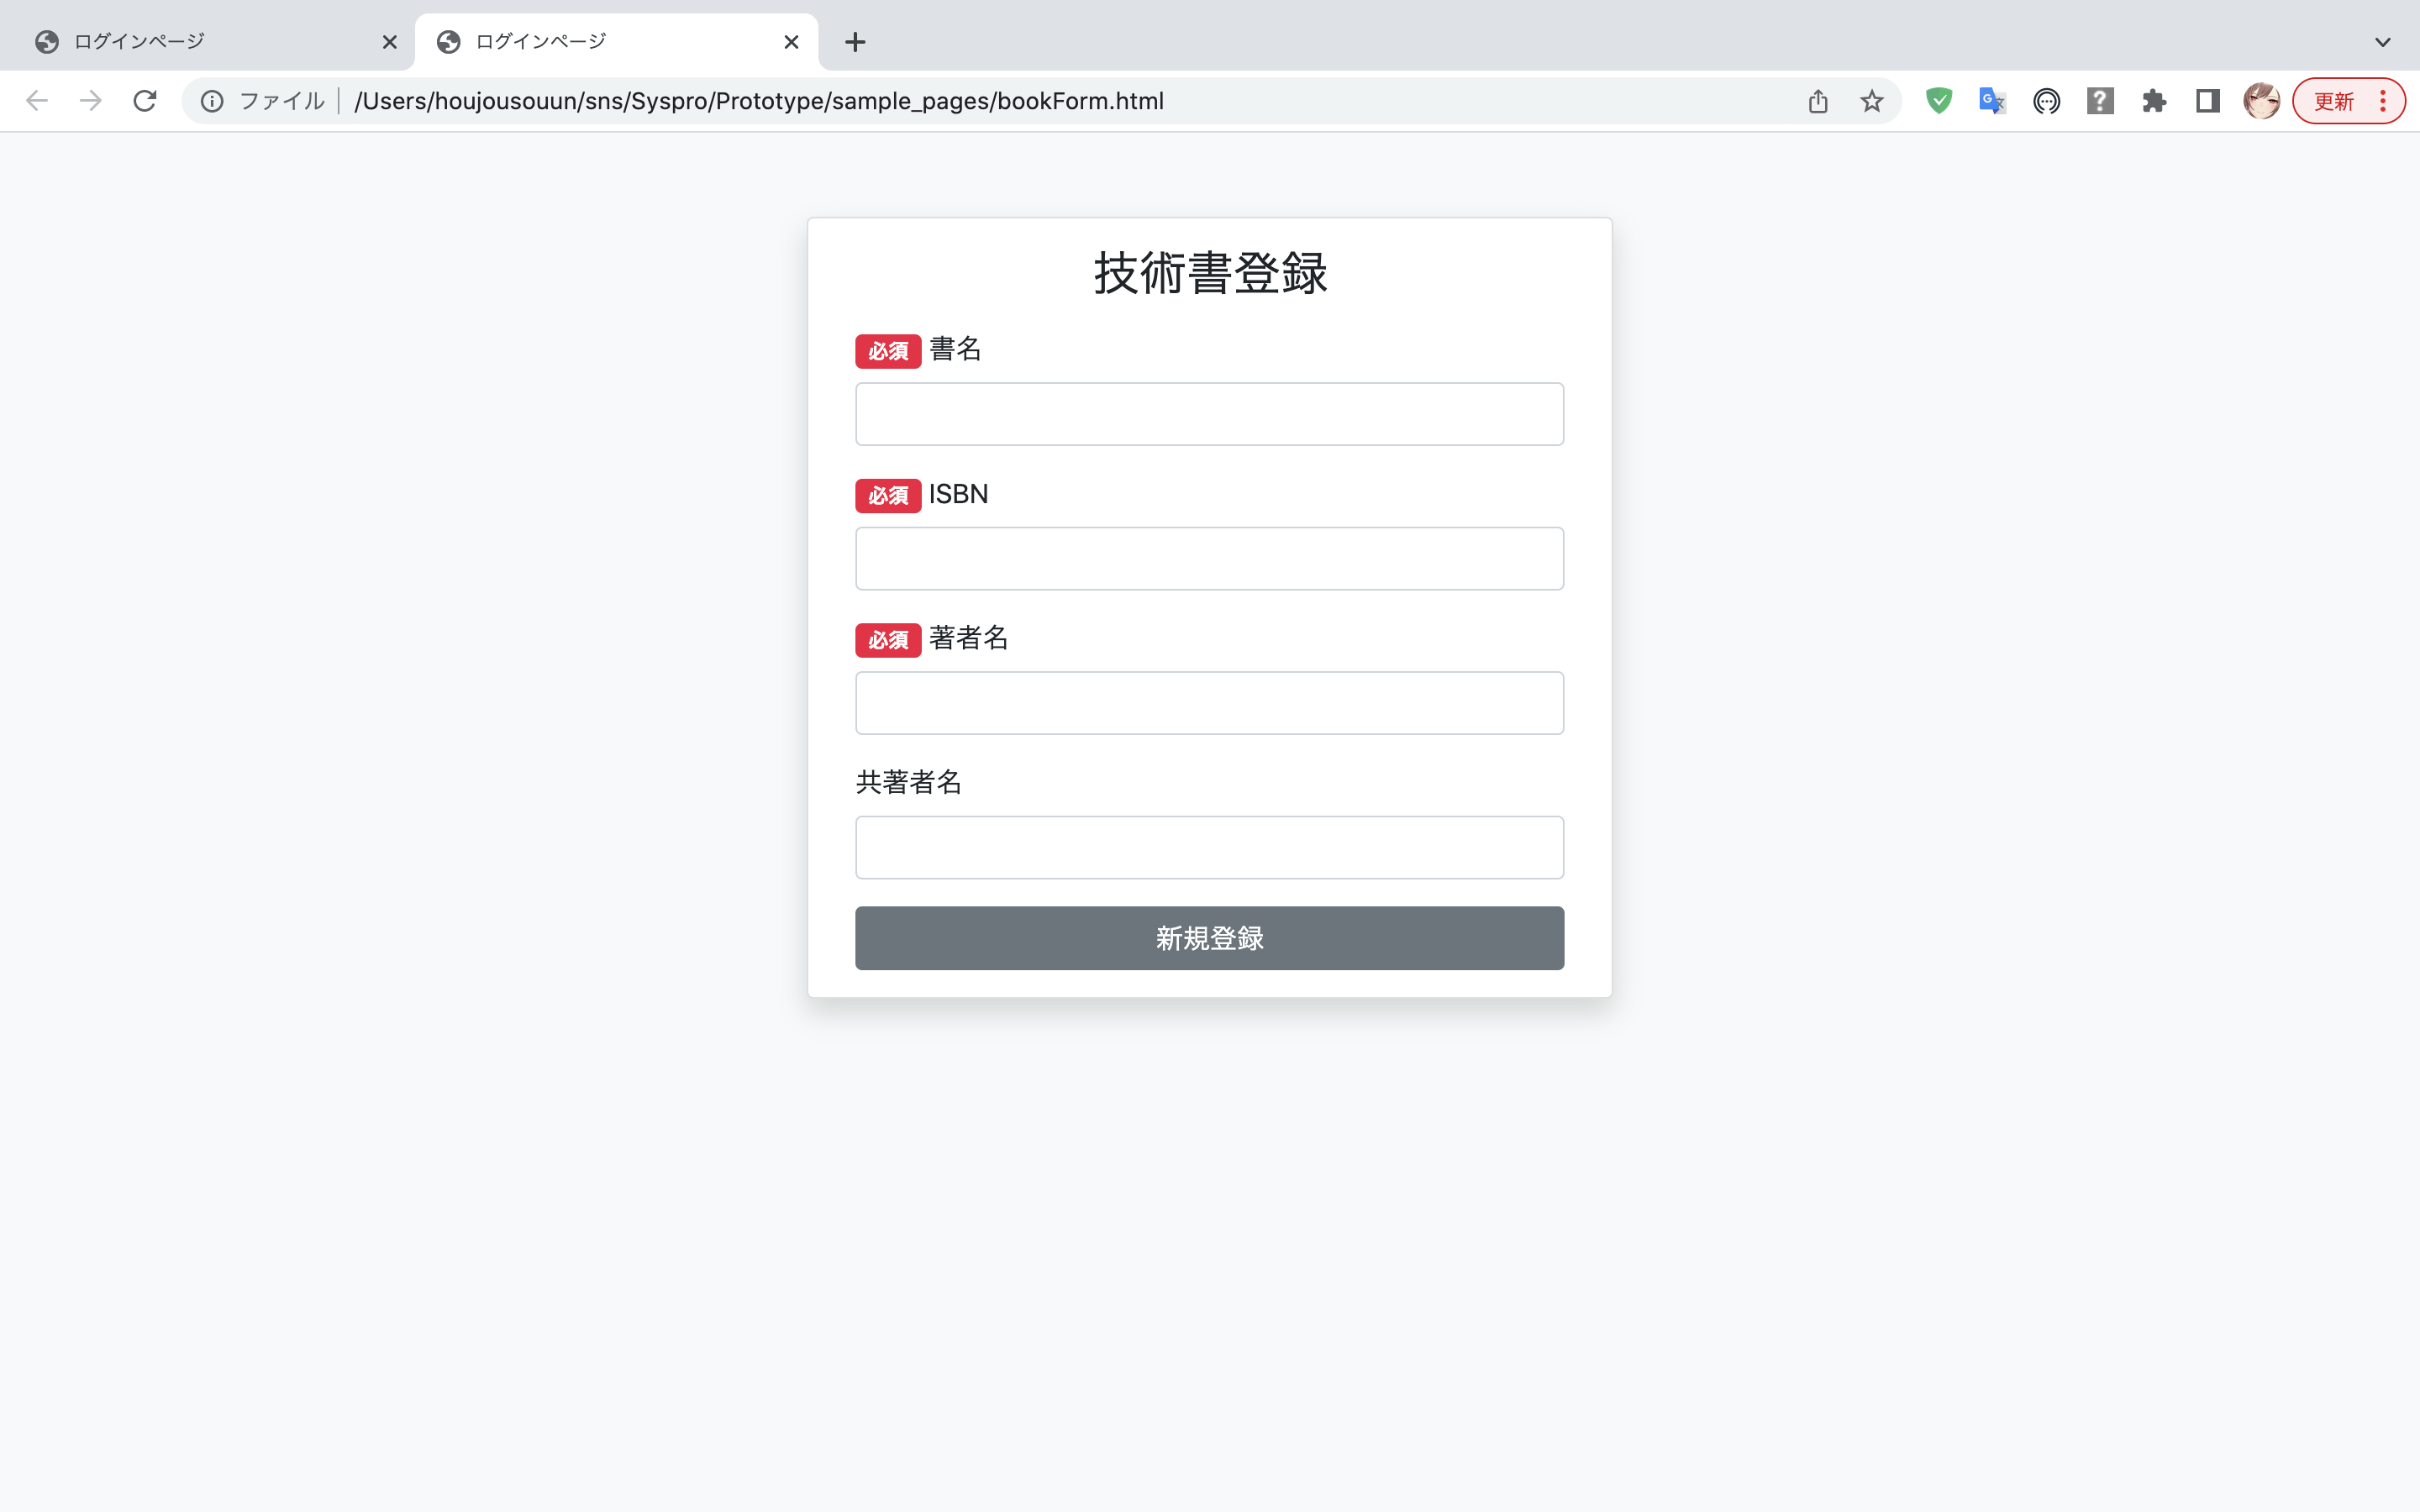
\includegraphics[scale=0.3,clip]{pictures/bookForm.png}
        \end{center}
    \end{figure}

    \begin{figure}[H]
        \begin{center}
            \caption*{commentForm.html}
            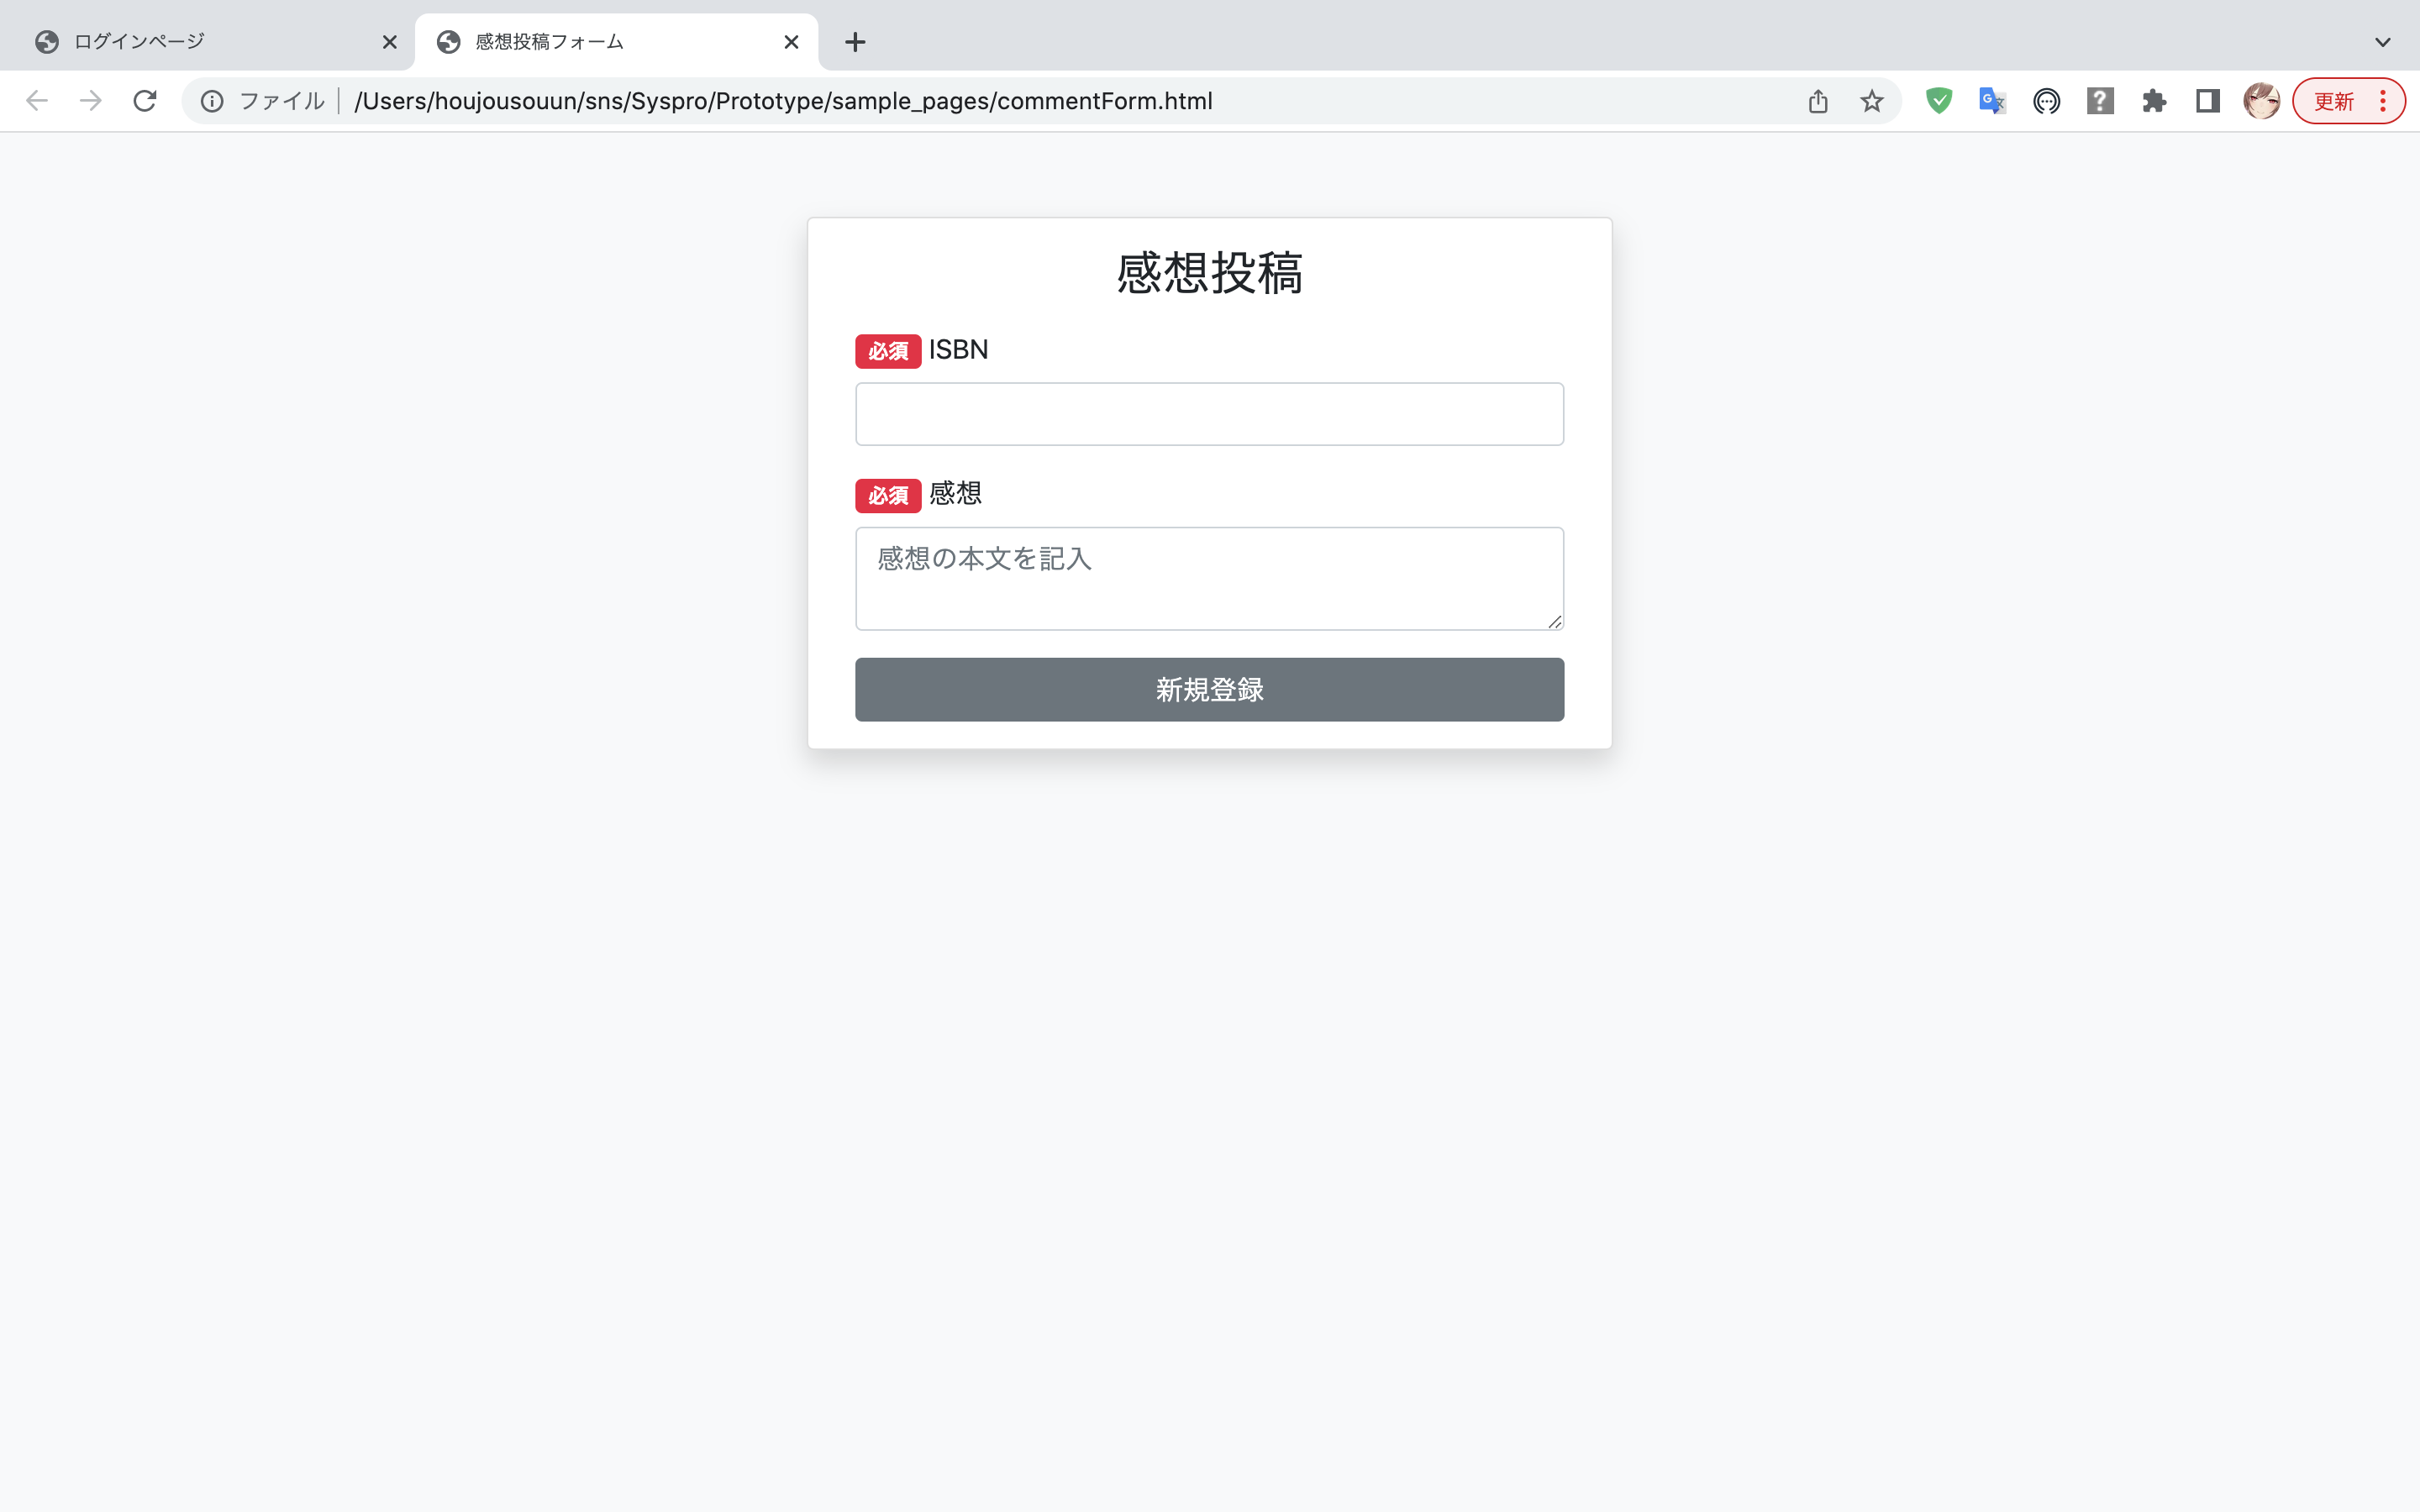
\includegraphics[scale=0.3,clip]{pictures/commentForm.png}
        \end{center}
    \end{figure}


    \section*{概念クラス図}
    \subsection*{\rm{作成者:實藤(フロントエンド担当)}}
    \begin{figure}[H]
        \begin{center}
            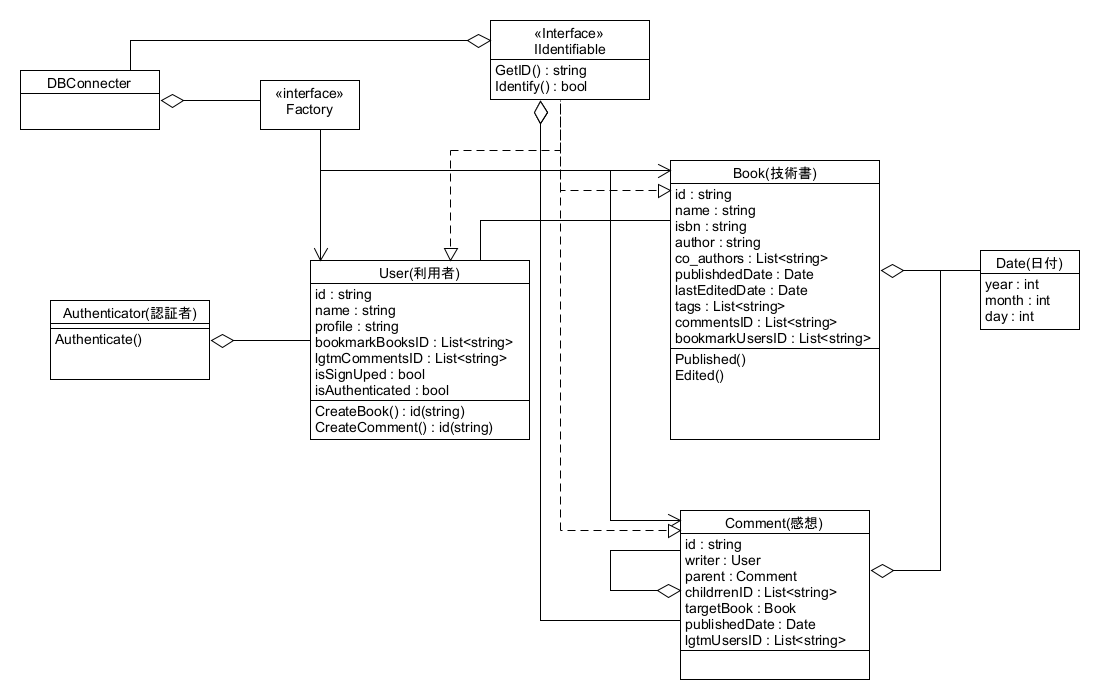
\includegraphics[scale=0.4,clip]{pictures/SysPro-ModelClassImage.png}
        \end{center}
    \end{figure}

    \newpage

    \section*{詳細クラス図}
    \subsection*{\rm{作成者:實藤(フロントエンド担当)}}
    \begin{figure}[H]
        \begin{center}
            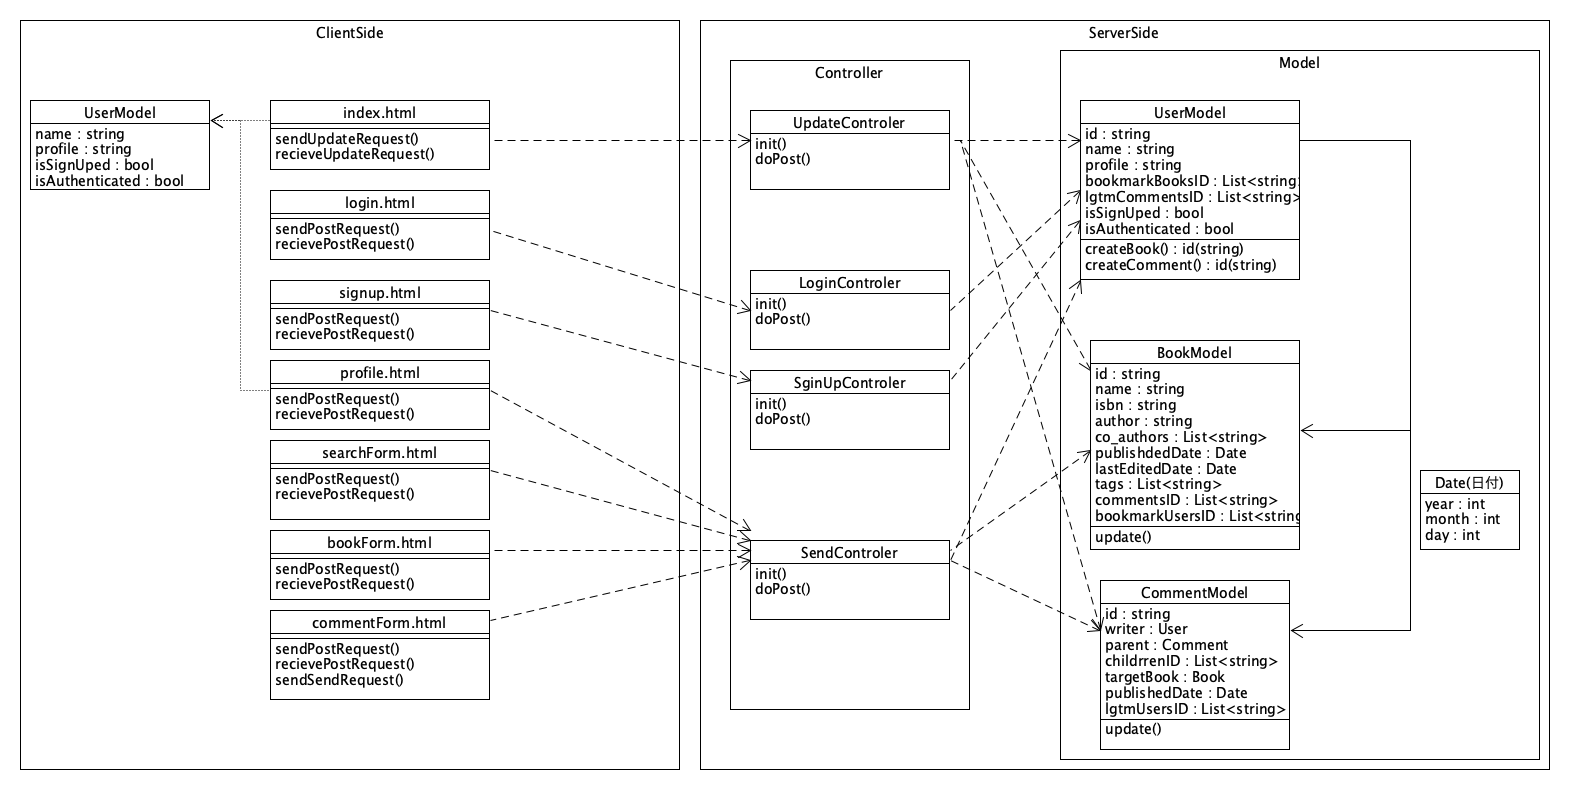
\includegraphics[scale=0.3,clip]{pictures/MVC.png}
        \end{center}
    \end{figure}

    \newpage

    \section*{シーケンス図}
    \subsection*{\rm{作成者:穂積(バックエンド担当)}}
    \begin{figure}[H]
        \begin{center}
            \caption*{アカウントを登録する}
            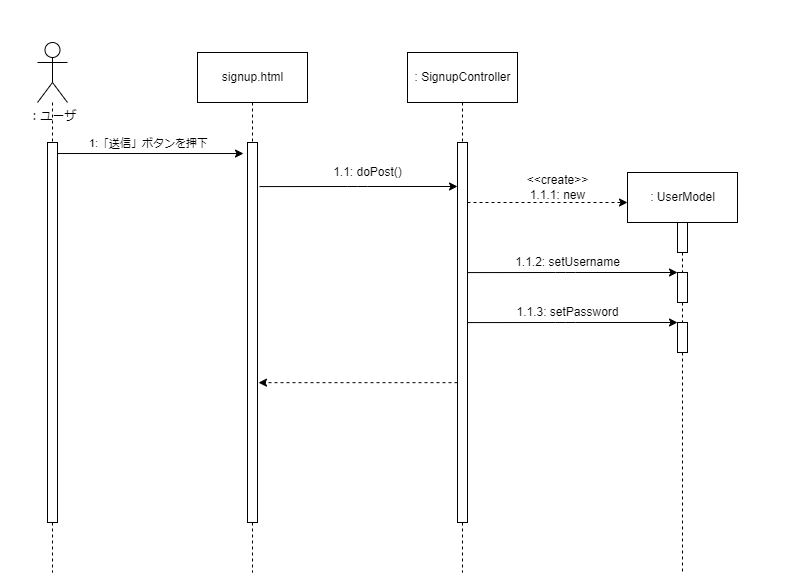
\includegraphics[scale=0.6,clip]{pictures/sequence-graph/signup.png}
        \end{center}
    \end{figure}

    \begin{figure}[H]
        \begin{center}
            \caption*{アカウントにログインする}
            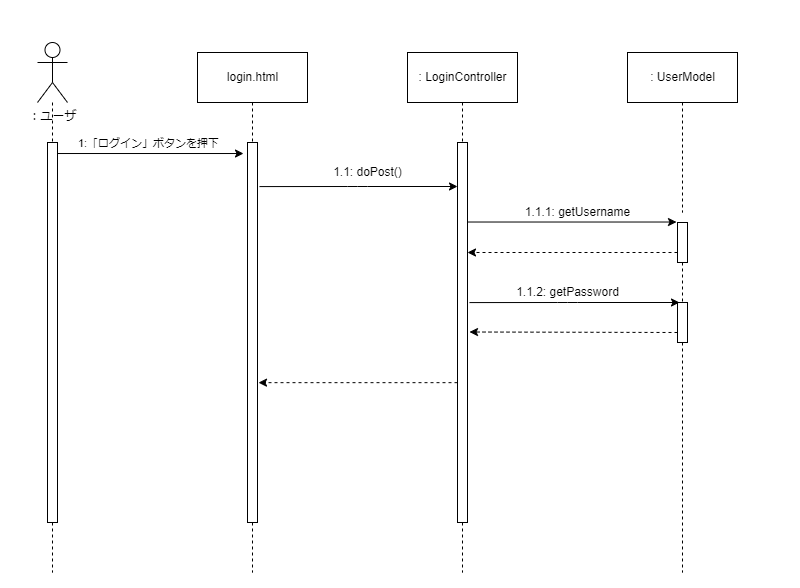
\includegraphics[scale=0.6,clip]{pictures/sequence-graph/login.png}
        \end{center}
    \end{figure}

    \begin{figure}[H]
        \begin{center}
            \caption*{技術書に関して投稿する}
            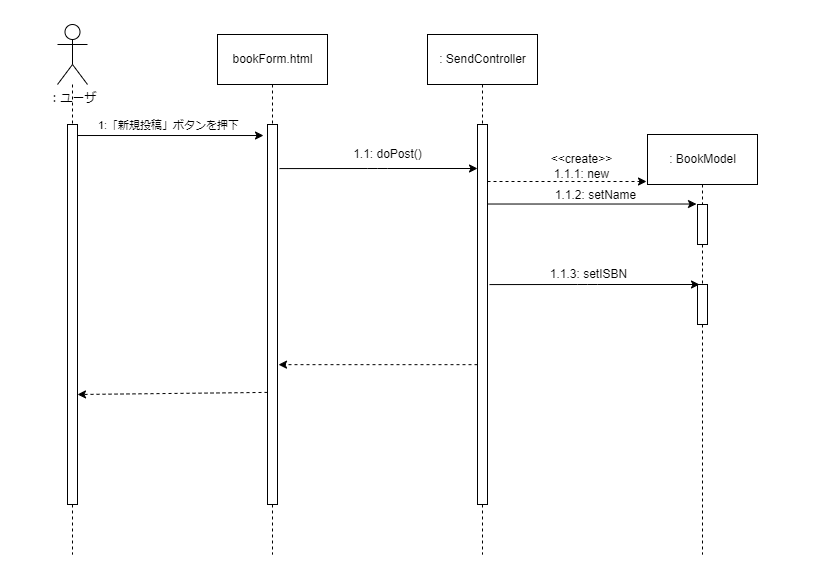
\includegraphics[scale=0.6,clip]{pictures/sequence-graph/sendAboutBook.png}
        \end{center}
    \end{figure}

    \begin{figure}[H]
        \begin{center}
            \caption*{技術書に関する投稿を閲覧する}
            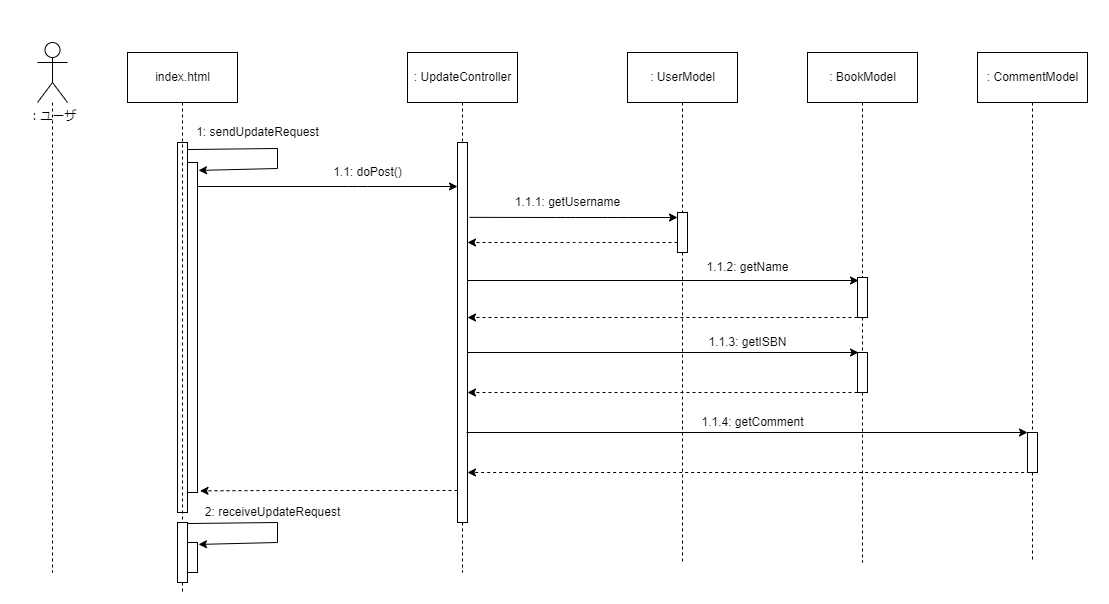
\includegraphics[scale=0.45,clip]{pictures/sequence-graph/watchMessages.png}
        \end{center}
    \end{figure}

    \begin{figure}[H]
        \begin{center}
            \caption*{他人の投稿に対して反応する}
            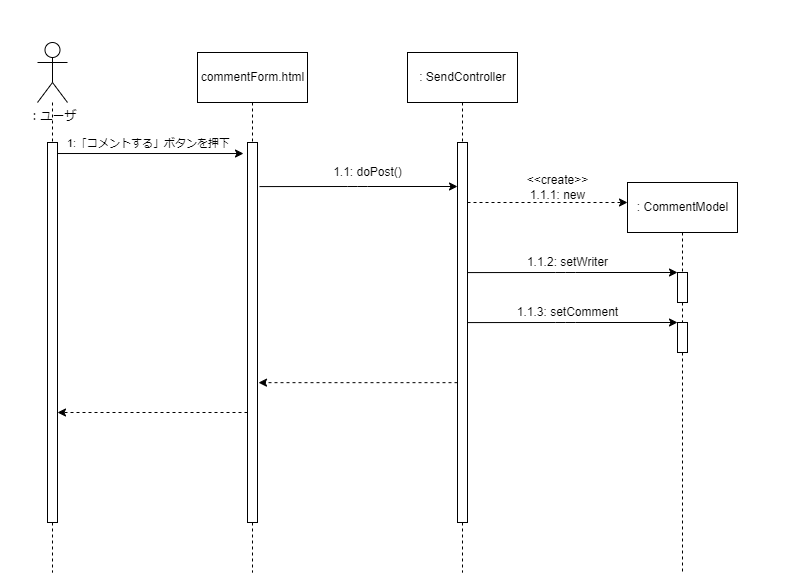
\includegraphics[scale=0.6,clip]{pictures/sequence-graph/reaction.png}
        \end{center}
    \end{figure}

    \begin{figure}[H]
        \begin{center}
            \caption*{技術者を検索する}
            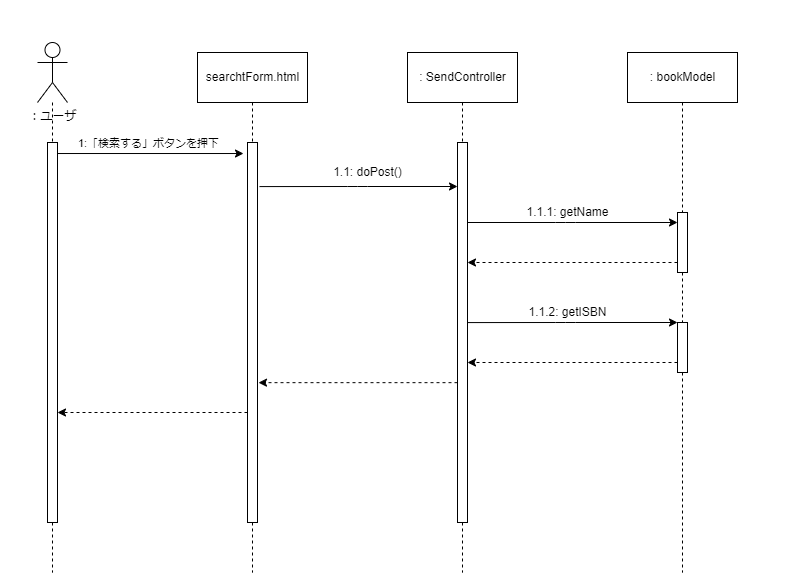
\includegraphics[scale=0.6,clip]{pictures/sequence-graph/searchBook.png}
        \end{center}
    \end{figure}

\end{document}